\section{Evaluation}
\label{sec::chp6::evaluation}

This section evaluates the \deeid system using the framework proposed by Bonneau \etal\ in \textit{The Quest to Replace Passwords}~\cite{bonneau_quest_2012}. The framework assesses authentication schemes across three key dimensions: usability, deployability, and security. Figure~\ref{fig:deeIDComp} visually compares \deeid with other authentication schemes, and here, we systematically analyse how \deeid meets or falls short of each evaluation criterion, acknowledging its strengths and limitations.

\begin{figure*}[h]
    \centering
    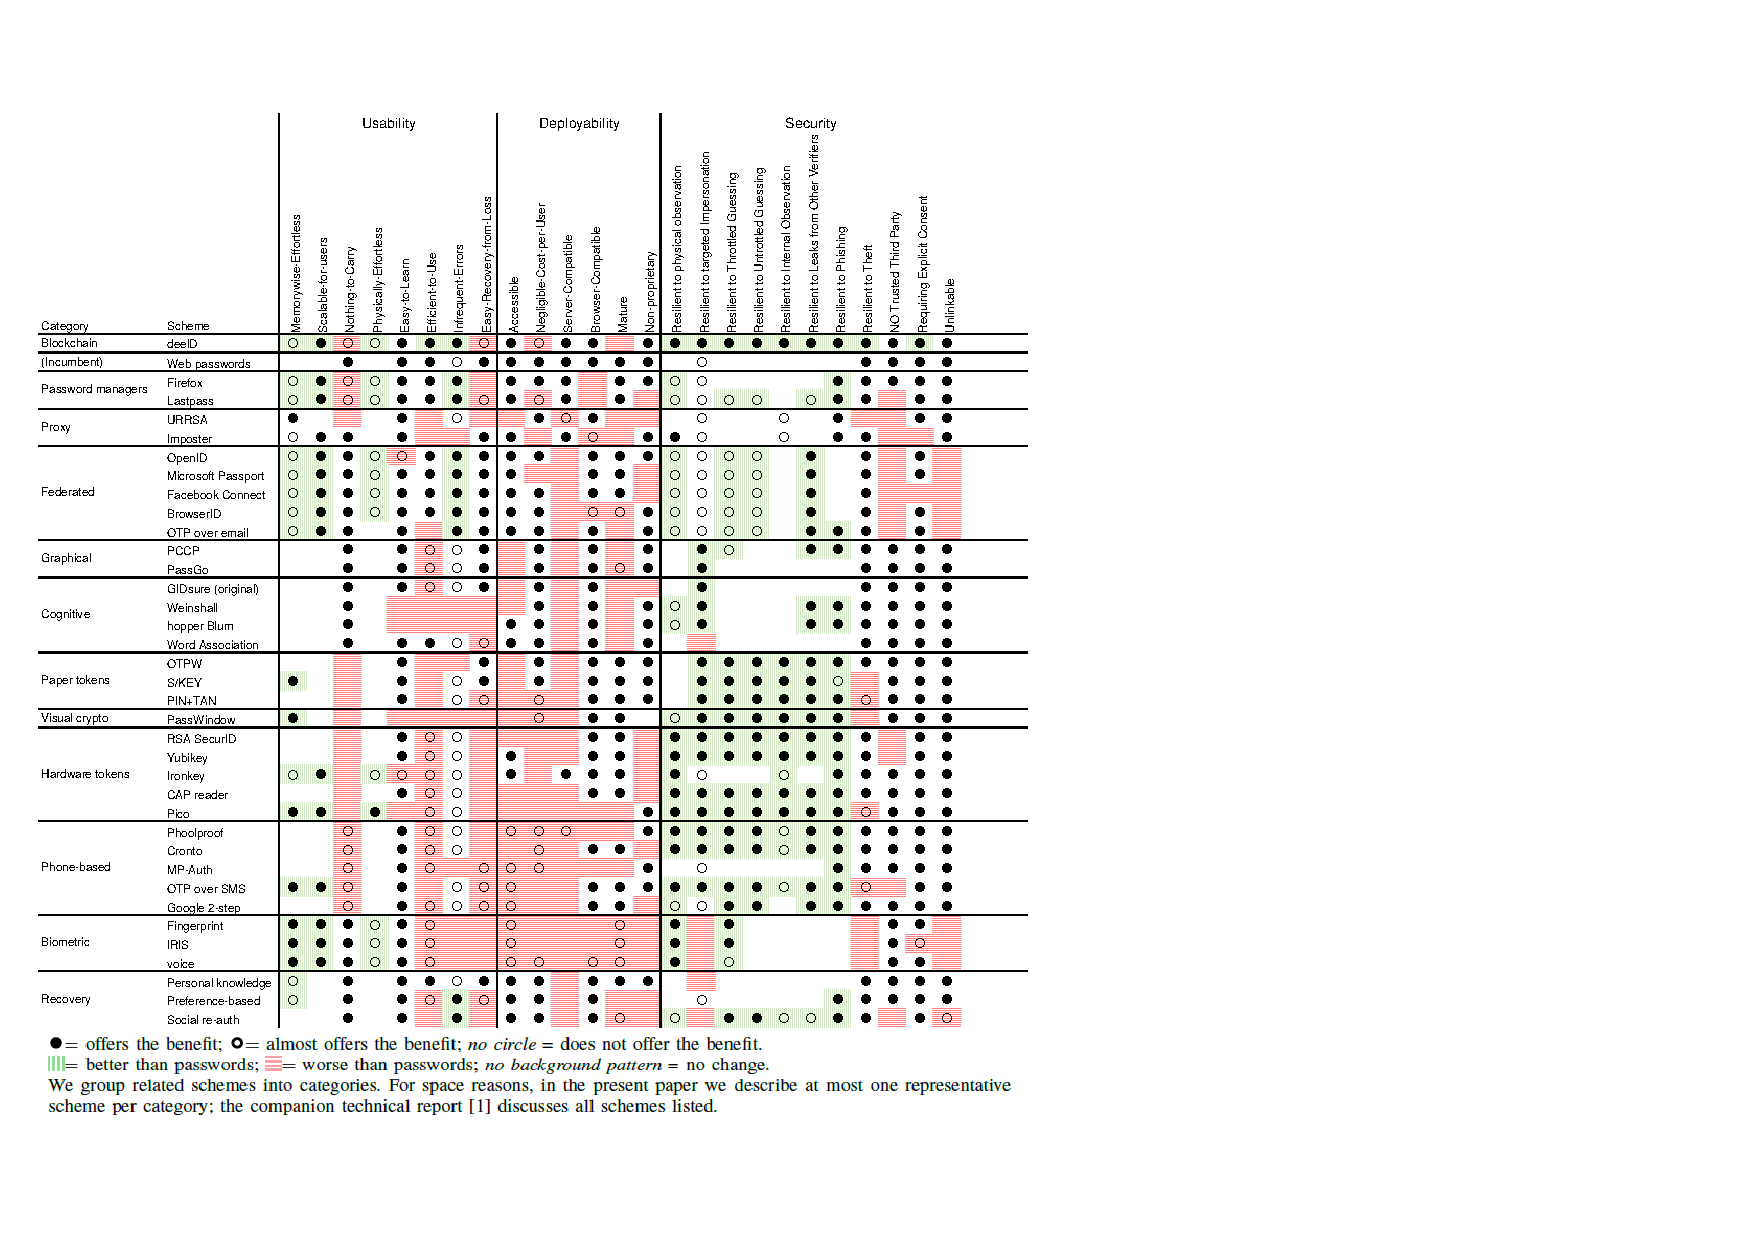
\includegraphics[trim={0 2cm 12cm 1cm},clip, scale=1]{figs/deeid/deeIDComparisonTable3.pdf}
    \caption{Visual evaluation of various schemes and our new blockchain-based scheme (\deeid).}
    \label{fig:deeIDComp}
\end{figure*}

\subsection{Usability Benefits}

\begin{enumerate}
    \item \textbf{Memorywise-Effortless}: There is no need for users to memorise passwords or other secrets; \deeid relies on a mobile phone device to store cryptographic secrets. This reduces cognitive load compared to traditional password systems. This benefit is similar to WebAuthn/Passkeys or password managers. However, the users may need to use a PIN to unlock their device.

    \item \textbf{Scalable-for-Users}: \deeid supports unlimited credentials and users can have multiple identities (issued from different organisations) without additional complexity. With the current system, there is a cost associated with transactions with the blockchain. Whilst this is a limitation of our method it is a technical challenge to overcome in future work. This benefit is similar to WebAuthn/Passkeys in regards to authentication.

    \item \textbf{Physically-Effortless}: Authentication and identification with \deeid requires scanning a QR code and pressing a button to confirm, a process that is physically straightforward and comparable to tapping a contactless card. There is a reliance on a mobile phone device and having it with you.

    \item \textbf{Easy-to-Learn}: \deeid is designed to be intuitive with minimal cognitive overhead. The actions and processes are familiar, such as scanning QR codes. The blockchain element is not easy to learn and most users are not required to learn or understand it; it can be abstracted away. Identity providers can provide onboarding and initial training if required.

    \item \textbf{Efficient-to-Use}: Authentication and identification is streamlined, requiring only a QR code scan and a single button press, making it faster than typing passwords or answering security questions. Compared to multi-factor authentication methods that involve multiple steps, \deeid offers a more efficient user experience. Network latency during blockchain queries may introduce minor delays.

    \item \textbf{Infrequent-Errors}: \deeid is reliable and deterministic. However, users would require their mobile phone device with them. Blockchain network issues might introduce errors or inconvenience.

    \item \textbf{Easy-Recovery-from-Loss}: This is a significant limitation of \deeid; there is no robust recovery mechanism. If a user loses their mobile device then they would not be able to recover their identity without backups. Users would need to get their identity re-issued from their providers.
\end{enumerate}


\subsection{Deployability Benefits}

\begin{enumerate}
    \item \textbf{Accessible}: The aim is to match or go beyond password's accessibility. Mobile phone devices are ubiquitous and most users have access to these devices with capability of securing cryptographic secrets on the hardware.  Accessibility is therefore high.

    \item \textbf{Negligible-Cost-per-User}: Blockchain transactions can incur charges, such as for issuing identities or updating contracts. The user requires a mobile phone which can be costly. Beyond these costs, all identity verifications and authentications have no costs associated with them.

    \item \textbf{Server-Compatible}: Compatibility with existing tech stacks were a key requirement in the design stage. \deeid requires no specialised server-side infrastructure unless a blockchain needs to be installed. Most organisations would be able to implement the password-less authentication feature easily. 

    \item \textbf{Browser-Compatible}: Do users need client change or additional software? It would be quasi-compatible if it reliance on common plugins like Flash. \deeid is a compatible with most modern browsers.

    \item \textbf{Mature-Technology}: \deeid uses mature technologies as the building block, however in itself it is not a mature technology or widely adopted. Maturity and adoption of this \deeid requires recognition amongst large technology organisations that control distribution.

    \item \textbf{Non-Proprietary}: This is where anyone can implement or use the scheme without royalties (not protected by patent or trade secrets). \deeid is designed and developed on open technologies such as Ethereum, the Fiat--Shamir cryptosystem, and other widely available client-server technologies.
\end{enumerate}


\subsection{Security Benefits}

\begin{enumerate}
    \item \textbf{Resilient-to-Physical-Observation}: No secrets are displayed or entered during authentication. The QR code displayed can be timed or randomised at a rapid rate. All operations occur on the user's device. The zero-knowledge properties of the protocols used means no secret information is revealed.

    \item \textbf{Resilient-to-Targeted-Impersonation}: Skilled or well-resourced malicious actors would not be able to impersonate the user unless the user's mobile phone device is stolen and the attacker can access it. \deeid is resilient against phishing attacks and other social engineering attacks.

    \item \textbf{Resilient-to-Throttled-Guessing}: Secrets are not stored on centralised servers, they are held on the user's device. It is computationally infeasible to attempt to guess the users's Fiat--Shamir secrets, especially with large key sizes.

    \item \textbf{Resilient-to-Unthrottled-Guessing}: Similar to throttled guessing, this is also unfeasible due to the nature of the cryptosystems used and lack of credential centralisation.

    \item \textbf{Resilient-to-Internal-Observation}: If a user interacts with a service on the client then they are secure against attacks, such as the Man-in-the-Browser malware. The users do not interact with the cryptographic secrets on the mobile phone, if stored on the secure enclaves then they are unobservable.

    \item \textbf{Resilient-to-Phishing}: The zero-knowledge nature of \deeid’s authentication ensures that no secret information is shared with verifiers. The operations on the mobile phone, where a service is authenticated, ensures that the user is unlikely to be phisehd.

    \item \textbf{Resilient-to-Theft}: The system is resilient-to-theft if a physical object cannot be used for authentication or identification by another user. It would be quasi-resilient-to-theft if protected by a PIN without rate control. \deeid is quasi-resilient-to-theft as the mobile phone device is likely to have a PIN or biometric. Future work can focus on making this aspect more secure.

    \item \textbf{No-Trusted-Third-Party}: \deeid uses a trusted third party to create an identity on the blockchain. Beyond this initial setup, \deeid does not use any other trusted third parties.

    \item \textbf{Requiring-Explicit-Consent}: Authentication and identification requires an explicit action from the user, such as scanning a QR code or pressing a button. This ensures authorised access and accidental or drive-by identification.

    \item \textbf{Unlinkable}: If the user is carrying out identification, then they are linkable due to their unique identity. However, if they carry out authentication (without the use of the blockchain), then it will be unlinkable, unless the services track the users by other means.
\end{enumerate}